\documentclass[a4paper,13.6pt]{article}
\usepackage{listings}
\usepackage{CJKutf8}
\usepackage{minted}
\usepackage{picinpar,graphicx}
\usepackage[utf8]{inputenc}
\usepackage[T1]{fontenc}
\usepackage{CJK}
\usepackage{geometry}
\author{langman}
\title{ACM-template}
\usepackage{lastpage}%获得总页数
\usepackage{fancyhdr}
\pagestyle{fancy}
%以下命令中L--左侧 R--右侧 C--中间 O--奇数页 E--偶数页
\fancyhead[LO,RE]{SHU--langman}%奇数页左侧,偶数页右侧显示页眉
\fancyfoot[CO,RE]{practice making surprise}%奇数页中间,偶数页右侧页脚为空
\fancyfoot[LO,CE]{}%奇数页左侧,偶数页中间页脚为空
\fancyfoot[RO,LE]{\thepage\ of
\pageref{LastPage}}%奇数页右侧,偶数页左侧显示 当前页 of 总页数
\renewcommand{\headrulewidth}{0.4pt}%改为0pt即可去掉页眉下面的横线
\renewcommand{\footrulewidth}{0.4pt}
\geometry{left = 2.5cm,right = 2.5cm,top = 2.5cm,botton = 2.5cm}
\begin{document}
\maketitle
\vspace{3cm}
\begin{CJK}{UTF8}{gbsn}
    \begin{figure}[!htb]
      \begin{center}
        
\includegraphics[width=0.80\linewidth]{../scoure/tupian.jpg}
        \caption{stay hungry stay foolish}
      \end{center}
    \end{figure}
\newpage

\tableofcontents
\newpage
\section{头文件}
\inputminted{c++}{../scoure/head.cpp}
\newpage
\section{图论}
\subsection{二分图}
判断是否二分图
\inputminted{c++}{../scoure/Graph_theory/pan2fen.cpp}
求出最大匹配数
\inputminted{c++}{../scoure/Graph_theory/2fentu.cpp}
\subsection{并查集}
\inputminted{c++}{../scoure/Graph_theory/bingchick.cpp}
\newpage
\subsection{最短路}
两种算法 但是要注意dijkstra无法处理负边的情况
\subsubsection{dijkstra}
需要注意的在于 可以更优化 我没写了 而且需要注意重边的情况
\inputminted{c++}{../scoure/Graph_theory/dijkstra.cpp}
\subsubsection{spfa}
需要注意的是怎么建边 双向边?
\inputminted{c++}{../scoure/Graph_theory/spfa.cpp}
\subsubsection{Flody}
这个就不写了,一个小dp
\subsection{最小生成树}
这是个什么玩意呢 图里面是吧,找到n-1条边使得生成一颗树,然后他的边权之和最小
\inputminted{c++}{../scoure/Graph_theory/prime.cpp}
\subsection{最大流}
\subsubsection{Dinic}
板子先存着,坑定用的着
\inputminted{c++}{../scoure/Graph_theory/dinic.cpp}
\newpage
\section{字符串}
\subsection{kmp}
适用点:\\
这个主要用在,一个是:他的那个周期函数的运用.一个是那个单模板串,多个匹配串的形式.
最主要的运用就是他的那个失配函数的运用.这里就随便弄一个板子过来了,为了打的快一点.
\inputminted{c++}{../scoure/date/kmp.cpp}
\subsection{字典树}
这个是一个比较高级的东西,一般这个玩意和前缀有点关系.
\inputminted{c++}{../scoure/date/Trie.cpp}
\subsection{ac自动机}
呦呦呦这个就高级了,他是基于那两个东西,字典树和kmp所衍生出来的一个算法.
\inputminted{c++}{../scoure/date/aczidongji.cpp}
\section{常用数据结构}
\subsection{STL}
\inputminted{c++}{../scoure/date/duilie.cpp}
\subsection{单调栈}
\inputminted{c++}{../scoure/date/dandianzhan.cpp}
\subsection{莫队算法}
处理的东西主要是在于区间,这里的区间不是单纯区间,而是你可以向上向下走的问题,并且有O(1)的递推式就可以走,这里的关键在于玄学把复杂度降到$N^{\frac{3}{2}}$然后需要处理的就是你走所带来的一个权值变化,这个是关键的问题
\inputminted{c++}{../scoure/date/mudui.cpp}
\subsection{点分治}
现在还不是很熟,所以放了一道例题,就是给你这个树让你去算这棵树上点对的距离小于等于k。
\inputminted{c++}{../scoure/date/dian_fen.cpp}
\subsection{树状数组}
适用于的方面是,单点更新,多次查询。
\inputminted{c++}{../scoure/date/treevector.cpp}
\subsection{前缀和}
适用于多次区间更新,一次查询,代码就不搞上去了。
\subsection{线段树}
现在的我对于这方面还不够熟悉,先留个板子
\inputminted{c++}{../scoure/date/treexian.cpp}
\subsection{高精度}
我个人习惯使用Java。就是怎么说呢,感觉要学会用自动补全以及几个常用的加减乘除
加add减sub乘mul除div模mod就很ok,然后那个大叔据都是从字符串转过来的,要熟悉一下字符串的一些常用函数.
\inputminted{java}{../scoure/date/bigjing.java}
\section{数学方面}
\subsection{常见公式}
\begin{enumerate}
\item 约数定理 若$n=\prod_{i=1}^kp_i^{a_i}$

\begin{enumerate}
\item 约数个数$f(n)=\prod_{i=1}^k(a_i+1)$
\item 约数和$g(n)=\prod_{i=1}^k(\sum_{j=0}^{a_i}p_i^j)$
\end{enumerate}

\item 小于$n$且互素的数之和为$n\varphi(n)/2$

\item 若$gcd(n,i)=1$,则$gcd(n,n-i)=1(1\leq i\leq n)$

\item 错排公式:$D(n)=(n-1)(D(n-2)+D(n-1))=\sum_{i=2}^n\frac{(-1)^kn!}{k!}=[\frac{n!}{e}+0.5]$

\item 威尔逊定理:$p\ is\ prime\ \Rightarrow (p-1)!\equiv-1(mod\ p)$

\item 欧拉定理:$gcd(a,n)=1\Rightarrow a^{\varphi(n)}\equiv1(mod\ n)$

\item 欧拉定理推广:$gcd(n,p)=1\Rightarrow a^n\equiv a^{n\%\varphi(p)}(mod\ p)$

\item 素数定理:对于不大于n的素数个数$\pi(n)$,$\lim\limits_{n\to\infty}\pi(n)=\frac{n}{\ln n}$

\item 位数公式:正整数$x$的位数$N=log10(n)+1$

\item 设$a>1,m,n>0$,则$gcd(a^m-1,a^n-1)=a^{gcd(m,n)}-1$

\item $[n = 1] = \sum_{d|n}u(d)$

\item $\sum_{d|n}\phi(d) = n$

\item 若$gcd(m,n)=1$,则:

\begin{enumerate}
\item 最大不能组合的数为$m*n-m-n$
\item 不能组合数个数$N=\frac{(m-1)(n-1)}{2}$
\end{enumerate}
\item 若$gcd(m,n)=1$,则:

\begin{enumerate}
\item 最大不能组合的数为$m*n-m-n$
\item 不能组合数个数$N=\frac{(m-1)(n-1)}{2}$
\end{enumerate}

\item $(n+1)lcm(C_n^0,C_n^1,...,C_n^{n-1},C_n^{n})=lcm(1,2,...,n+1)$

\item 若$p$为素数,则$(x+y+...+w)^p\equiv x^p+y^p+...+w^p(mod\ p)$

\item NTT常用素数

\begin{tabular}{cccc}
    \hline
    $r⋅2^k+1$&$r$&$k$&$g$\\
    \hline
    3&1&1&2\\
    5&1&2&2\\
    17&1&4&3\\
    97&3&5&5\\
    193&3&6&5\\
    257&1&8&3\\
    7681&15&9&17\\
    12289&3&12&11\\
    40961&5&13&3\\
    65537&1&16&3\\
    786433&3&18&10\\
    5767169&11&19&3\\
    7340033&7&20&3\\
    23068673&11&21&3\\
    104857601&25&22&3\\
    167772161&5&25&3\\
    469762049&7&26&3\\
    998244353&119&23&3\\
    1004535809&479&21&3\\
    2013265921&15&27&31\\
    2281701377&17&27&3\\
    3221225473&3&30&5\\
    75161927681&35&31&3\\
    77309411329&9&33&7\\
    206158430209&3&36&22\\
    2061584302081&15&37&7\\
    2748779069441&5&39&3\\
    6597069766657&3&41&5\\
    39582418599937&9&42&5\\
    79164837199873&9&43&5\\
    263882790666241&15&44&7\\
    1231453023109121&35&45&3\\
    1337006139375617&19&46&3\\
    3799912185593857&27&47&5\\
    4222124650659841&15&48&19\\
    7881299347898369&7&50&6\\
    31525197391593473&7&52&3\\
    180143985094819841&5&55&6\\
    1945555039024054273&27&56&5\\
    4179340454199820289&29&57&3\\
    \hline
\end{tabular}
\end{enumerate}
\subsection{三个特别的数}
\subsubsection{Fib 数列}
$f(x) = f(x-1)+f(x-2)$ \qquad $f(0) = 0,f(1) = 1$
\subsubsection{卡特兰 数}
$\sum_{i=1}^n f_i*f_{n-i}=f_n$ \qquad
$h(n) = C_{2n}^n - C_{2n-1}^{n}$
注意它这个数字来自于什么情况。
\subsubsection{斯特林公式}
$\sqrt{2*PI*n} * (\frac{n}{e})^n = n!$
\subsubsection{伯努力数}
这个数的定义来自于,之前人们对自然数幂的求解的过程中,出现的一种操作,感觉这个的主要目的在于求有关自然数幂和的问题上,所有的问题都不是直接给出的,多点见识。\\
$\sum_{i=1}^n i^k = \frac{1}{k+1}*\sum_{i = 1}^{k+1}C_{k+1}^i*B_{k+1-i}*(n+1)^i$ \qquad $B_0 = 1,\sum^n_{k = 0}C_{n+1}^k*B_k = 0$ \\ $B_n = -\frac{1}{n+1}\sum_{i=1}^{n-1}C_{n+1}^i*B_i$
下面是一个求自然数幂和的板子
\inputminted{c++}{../scoure/math/bo.cpp}
\subsection{数论}
第一个自然是最基础的欧几里得算法,欧几里得算法的用处有很多,求最大公倍数,解方程,很多。在后面的过程会把一些常见的板子列出来,一般来说这些板子
都已经经过验证,但是不好说对吧。简单题我们可以通过
一些模板直接得出答案,但是怎么说,这些对于难题
估计只能算工具,重要的是如何转换。
\subsubsection{高斯消元}
\inputminted{c++}{../scoure/math/guess.cpp}
\subsubsection{线性基}
\inputminted{c++}{../scoure/math/linner_base.cpp}
\subsubsection{素数}
素数筛法,线性筛
\inputminted{c++}{../scoure/math/shai.cpp}
\subsubsection{梅森素数}
一个知识点吧,m是一个正整数,且$2^m-1$为素数,那么m一定为素数。\\
如果m是一个素数,$M_p = 2^p-1$是梅森数\\
如果p是一个素数,并且$M_p = 2^p-1$也是素数,那么称$M_p$为梅森素数\\
对梅森素数的判定是一个算法:\\
Lucas-Lehmer:
$r_k \equiv r_{k-1} -2$\quad mod$M_p$\quad $r_1 = 4$
当且仅当 $r_{p-1} \equiv 0$\quad mod$M_p$
\subsubsection{miller-robin快速判素数}
\inputminted{c++}{../scoure/math/miller_robin.cpp}
\subsubsection{欧几里得}
\inputminted{c++}{../scoure/math/GCD.cpp}
然后是基于这个定理得出的一个定理,中国剩余定理
\inputminted{c++}{../scoure/math/chineseshengyu.cpp}
\subsubsection{乘法逆元}
思想是通过扩展欧几里得来得出,如果缘分到了,那么
还能用费马小定理来解,上面还有一个打表的方法O(n).
\inputminted{c++}{../scoure/math/niyuan.cpp}
\subsubsection{欧拉函数}
p为素数时$\phi(p) = p-1 $\\
a与n互质的时候 $a^{\phi(n)}\equiv 1$ mod $ n$\\
m,n互质$\phi(mn) = \phi(m) * \phi(n)$\\

这个东西好呀,他求的是比n小的,并且和n互质的数的个数
\inputminted{c++}{../scoure/math/oula.cpp}
更多的来说我觉得这个东西是一个工具,他对解一些题有很重要的作用,起到一个工具的作用
我目前学的比较浅,对他的优化作用没有很深的了解。几个定理\\
$\sum_{d|n}\phi(d) = n$ \qquad $\sum_{i=1}^n k_{gcd(k,n) = 1} = \frac{n*\phi(n)}{2}$
\subsubsection{莫比乌斯函数}
$F_n = \sum_{d|n}^n f_d$
$f_n = \sum_{d|n} u(d)*F(\frac{n}{d})$\\
$F_n = \sum_{n|d} f_d$
$f_n = \sum_{n|d} u(\frac{d}{n})*F(d)$\\
和欧拉函数一样很重要的一个函数他的定义我就不说了,毕竟我latex学的还不好,公式的
插入对我来说用处不大。
\inputminted{c++}{../scoure/math/mobius.cpp}
\subsubsection{二项式反演}
$f(n) = \sum_{k=0}^n C_n^k g(k)$
$g(n) = \sum_{k=0}^n (-1)^{n-k} C_n^k f(k)$
\newpage
\subsection{博弈}
\subsubsection{主要的解题思想}
官方说的是通过必败点和必胜点来判定
先通过必败点来推,直接来看必胜点,把问题抽象成图 把状态抽象成点,必败点就是先手必败点,然后通过必败点能走到的搞成必胜点,如过有一个状态没有走过 而且他后面的路都是必胜点那么他就是必败点。感觉就像dp一样,记忆化搜索。
当然题目不可能出的那么简单的。
不过根据雄爷定理,万事不离期宗,掌握基本,扩展自己去发掘。
\subsubsection{题型}
巴什博弈\\
这个是最简单的博弈,就是一堆东西,每个人自己能拿1-n件,谁最后一个拿完谁赢,这个是最简单的,不记录。
\\威佐夫博弈\\
有两堆各若干个物品,两个人轮流从某一堆或同时从两堆中取同样多的物品,规定每次至少取一个,多者不限,最后取光者得胜。
这个的解题思路在于通过前面的那个np问题来解决,用局势来思考这些问题,前几个局势在于(0,0),(1,2),(3,5),(4,7).....然后一些大佬就总结出了一些牛逼的结论$( a_k,b_k),a_k=\frac{k*(\sqrt{5}+1)}{2} , b_k=a_k+k$人才。
\\Fibonacci\\
有一堆个数为n的石子,游戏双方轮流取石子,满足:
\\(1)先手不能在第一次把所有的石子取完;
\\(2)之后每次可以取的石子数介于1到对手刚取的石子数的2倍之间(包含1和对手刚取的石子数的2倍)。 约定取走最后一个石子的人为赢家。
结论是 当n为Fibonacci数时,先手必败
\\尼姆博弈\\
有三堆各若干个物品,两个人轮流从某一堆取任意多的物品,规定每次至少取一个,多者不限,最后取光者得胜。
这个博弈有点意思 他的必败点的局势在于$(a,b,c) a \land {b \land c} = 0$
\subsubsection{SG函数}
这个在看之前感觉很高级但是啊,好像也就是一个dp的过程,通过一个必败点,看成起点然后,那个方法看成通向下一个起点的路,然后找所有能直接到这个必败点的必胜点。好像也就那么回事。好像能解决的都是小数字题这是一个板子,f里面存的是方法,多堆问题可以转化成异或来解决。
sg函数的定义是最小整数不属于,然后sg函数在一定程度上是存在一定的技巧,或者说是规律.我们就是需要去找哪些规律,一般都是转化成求异或的问题.
\inputminted{c++}{../scoure/math/boyi.cpp}
\subsubsection{解题策略}
* 1  :相信自己的第一感觉\\
* 2 :博弈都会和一些特别的数搭边 , 所以第一件事坑定是分析局势然后找找看是不是有特别的意义,像什么 卡特兰数,fib数列 ,幂次方,异或的值是否为0;\\
* 3  : 不挂怎么说,记得打表。\\
\subsection{组合数学}
\subsubsection{求组合数}
第一个是求组合数,方法很多不去列举,注意的是一般来说,组合数都是需要去
模一个数,所以他的分母在计算的时候是需要去求逆元的
\inputminted{c++}{../scoure/math/zuhe.cpp}
\subsubsection{polay定理}
设G={p1,p2,…,pt}是X={a1,a2,…,an}上一个置换群,用m种颜色对X中的元素进行涂色,那么不同的涂色方案数为
$$\frac{1}{G}\sum_{k=1}^t m^{Cyc(p_k)}$$
$Cyc(p_k)$是置换$p_k$的循环节个数
注意这里也是可以进行更改的,我们需要知道的是,对于每个循环节的意义是什么,这里要求的是每个循环节里面的颜色必须相同,这也就是为什么polay也是可以做到有条件的使用.我们要用有限的条件对这几个循环节进行赋值,这里的每一个循环节我可以理解成一个点,压缩点,对于限制条件,来看我这个群的操作是否可取
\subsubsection{Pell方程}
$$x^2-dy^2=1$$
当d不为平方数时,有无穷多的解。接下来是通项的推导
$$ x_{n+1} = x_1*x_n+d*y_1*y_n,y_{n+1} = x_1*y_n + y_1*x_n $$
暴力求$x_1,y_1$然后矩阵快速幂
\subsubsection{lucas定理}
当组合数的基数过大的时候进行这些操作但是注意,我们的操作也是要求那个模数为素数,且
模数要小的情况下,素数的情况我们可以用扩展lucas定理来解决。一个工具,一个数论上的分支。
\inputminted{c++}{../scoure/math/lucas.cpp}
\subsection{线代}
\subsubsection{bm求解n阶递推式}
\inputminted{c++}{../scoure/math/bm.cpp}
\subsubsection{fwt优化多项式乘法}
fft用的方面在于$f_n = \sum_{i+j=n}g_i*g_j$
fwt用的就是在于$f_n = \sum_{i^|&j ==n} g_i*g_j$
\inputminted{c++}{../scoure/math/fwt_ban.cpp}
\subsubsection{fft优化多项式乘法法}
这个是一个工具,他的作用是加速多项式得乘法。这个点得难处还是在于多项式的构建,其实也不是
非常复杂得东西,当然他的原理,不敢去碰。关键词:多项式乘法,并且复杂度为1e5左右。
\inputminted{c++}{../scoure/math/fft.cpp}
\subsubsection{ntt优化多项式}
用原根来处理多项式乘法,当数字过大的时候fft就有可能爆精度,ntt就有了用,这里需要注意的是使用条件,以及原根的取值
\inputminted{c++}{../scoure/math/ntt.cpp}
\subsubsection{矩阵快速幂}
这类方法,很多是用在递推关系式的时候,像什么fib数列什么的。
\inputminted{c++}{../scoure/math/ju_quick.cpp}
\subsubsection{矩阵方面知识}
就是用高斯消元法去解决一些问题,像什么秩和方阵的值。
\subsection{计算几何}
\subsubsection{一些定理}
\begin{enumerate} % 有序列表
    \item 笛卡尔定理: \\
    定义一个圆的曲率是$k = \frac{1}{r}$r是半径,若平面有两两相切,且有六个独立切点的四个圆,设其曲率分别为$k_1,k_2,k_3,k_4$(若该圆与其他圆均外切,则曲率取正,否则取负)则满足下面的性质:
    $$(k_1+k_2+k_3+k_4)^2 = 2*(k_1^2+k_2^2+k_3^2+k_4^2)$$
\end{enumerate}
\subsubsection{几何基本知识}
\emph{矢量}\\
矢量的乘积有很多的作用,注意定义。
适用点在于:1:面积 2:位置\\
\emph{跨立实验与判断两线段是否相交}\\
线段$P_1P_2,Q_1Q_2$,相交的条件为\\
$P_1Q_1$x$P_1P_2$  *  $P_1P_2$x$P_1Q_2>=0$\\
$Q_1P_1$x$Q_1Q_2$  *  $Q_1Q_2$x$Q_1P_2>=0$\\
\emph{pick定理}\\
线段上的是整数点的数的个数 求gcd;\\
PICK定理 设以整数点为顶点的多边形的面积为S,多边形内部的整数点数为N,多边形边界上的整数点数为L,则 S=L/2 + N-1

\subsubsection{判断点是否在多边形中}
\inputminted{c++}{../scoure/math/jihe.cpp}
为1的时候,则在内部。2,应该是边上。
\subsubsection{凸包问题}
\inputminted{c++}{../scoure/math/tubao.cpp}
\subsection{概率论}
目前做的题目比较少,有次做到过一题,他的解决方法是,对于期望问题,我们是先对子状态进行分析,再去求每个子状态的概率,和期望.思想在这个地方,要不然就是找规律.
\subsection{插值法}
拉格朗日插值法\\
这个是对于一个n次函数,我用n+1个点去确定的一种方法,相当于对于直线来说,我是两个点去确定这个玩意,但是现在我们是通过n+1个点去确定这个曲线
$$ L_n(x) = \sum_{i = 1}^n(\prod_{j=1,j \neq i}\frac{x-x_j}{x-x_i})*y_i$$
\inputminted{c++}{../scoure/math/lang.cpp}
牛顿插值法\\
这怎么说了,这个的好处在于我们不断对于一个函数进行加点的时候,不会导致之前的重新计算,好像也没什么用处
$$N_n(x) = f(x_0) + f(x_0,x_1)(x-x_0)+  .... +f(x_0,x_1,....,x_n)(x-x_0)(x-x_1)....(x - x_n)$$
$$ f(x_0,x_1...x_n) = \sum_{j = 0}^n(\frac{f_j}{\prod_{i =0,i \neq j}^n(x_j-x_i)} )$$
\section{状态转移 dp}
dp的定义:
1:记忆化搜索;2:状态转移
所以我们的解决方案总是跟着这个来走,从定义出发。
难点集中于两个方面,状态式的确定和状态转移方程的确定
\subsection{背包}
背包的问题主要以下几种:
01背包,部分背包,完全背包;[相对来说比较简单] ,分组背包[个人感觉较难]
背包难在如何, 确定维数,确定背包的容量是什么以及背包的价值是什么,还有背包的dp关系转移式。
\subsection{一些常见的dp}
\subsubsection{LIS 最长上升子序列}
\inputminted{c++}{../scoure/dp/longerxuelie.cpp}
\subsection{树形dp}
关键点在于找状态点间的关系,他一般只有三个关系,父亲节点
,儿子节点,还有兄弟节点,去找他们之间的关系,所以一般是两遍dfs
找父亲与儿子的关系,找儿子与父亲的关系。
\subsection{数位dp}
这个dp的精髓在于记忆化搜索,也就是在最高位不是被限定的情况下进行记录,这样的话省掉很多多余的步骤。
所有的出发点都处于这个目的。
\subsection{状压dp}
这个dp的精髓在于状态转移,不过能压缩的情况也是很限定的。
像什么每个点的状态在于都是能用两个状态来描述,且这些点不多,但是组合的方式很多。
一些状压dp经常用的上的公式。
\inputminted{c++}{../scoure/dp/zhuangtai.cpp}
\section{常用公式}
\subsection{杂}
\subsubsection{约瑟夫问题}
$n$个人围成一圈,从第一个开始报数,第$m$个将被杀掉
\begin{lstlisting}
int josephus(int n, int m)
{
    int r = 0;
    for (int k = 1; k <= n; ++k) r = (r + m) % k;
    return r + 1;
}
\end{lstlisting}
\subsection{积分以及求导}
  \begin{figure}[!htb]
      \begin{center}
        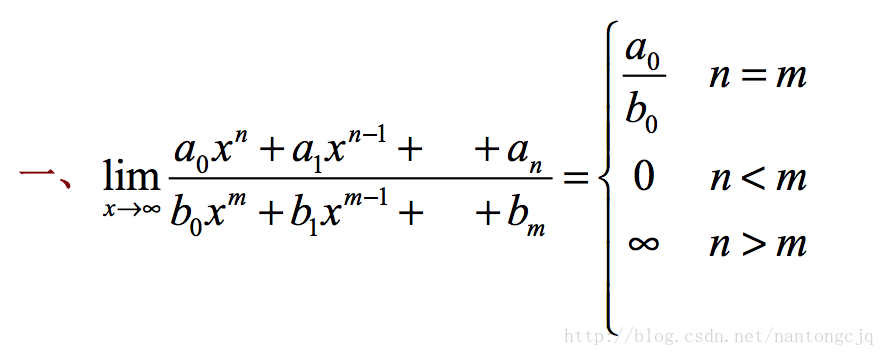
\includegraphics[width=0.50\linewidth]{../scoure/1.png}
      \end{center}
    \end{figure}
    \begin{figure}[!htb]
      \begin{center}
        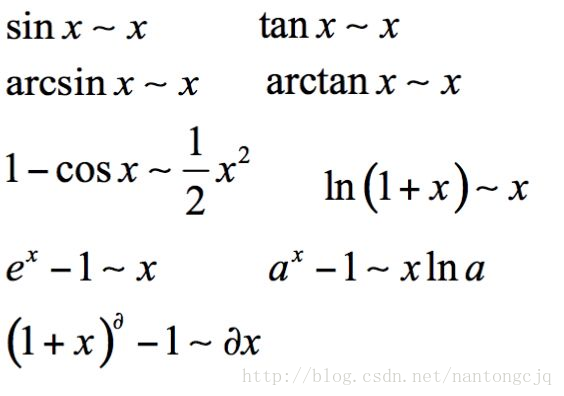
\includegraphics[width=0.30\linewidth]{../scoure/3.png}
      \end{center}
    \end{figure}
    \begin{figure}[!htb]
      \begin{center}
        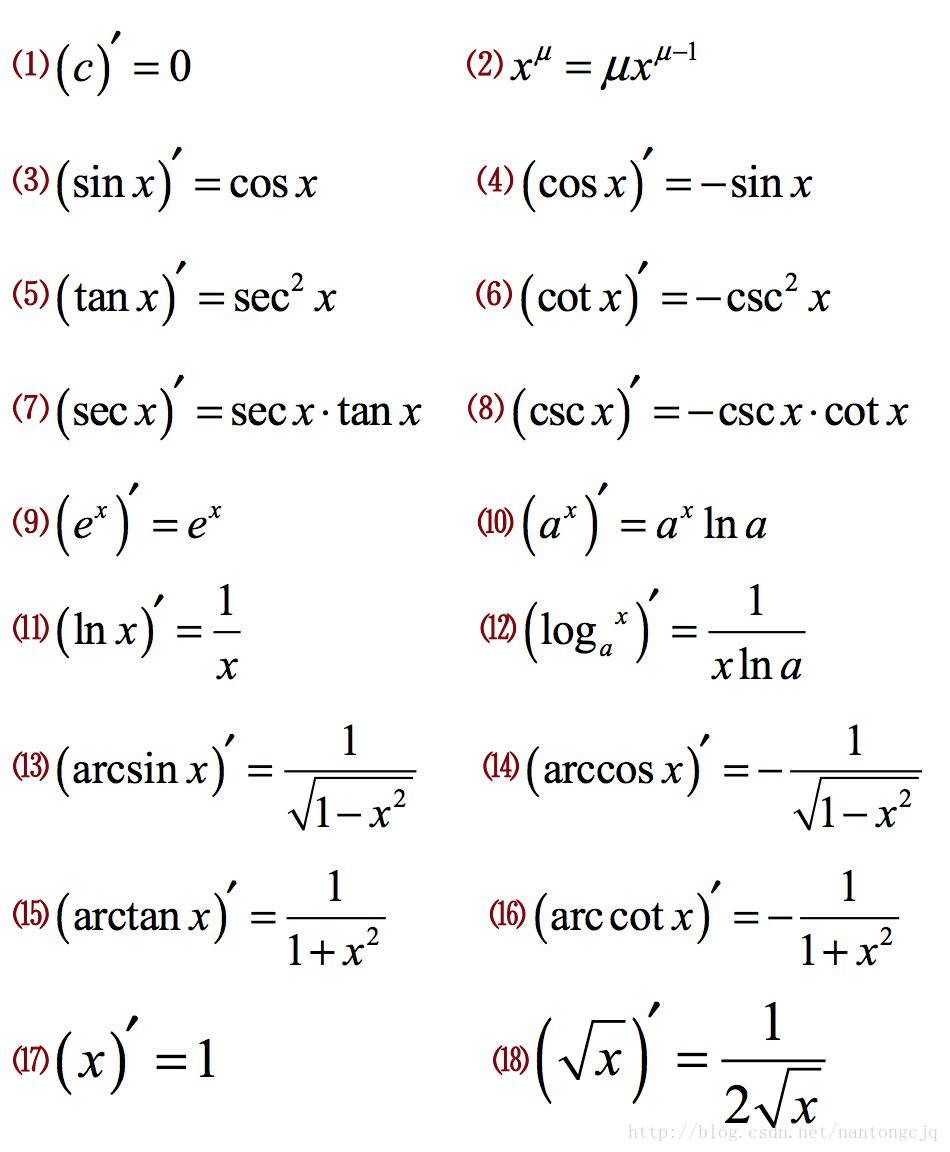
\includegraphics[width=0.50\linewidth]{../scoure/5.png}
      \end{center}
    \end{figure}
    \begin{figure}[!htb]
      \begin{center}
        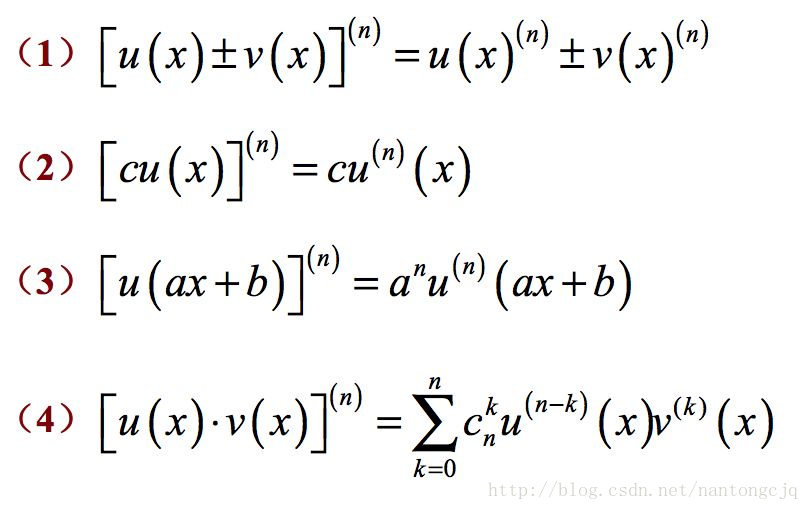
\includegraphics[width=0.50\linewidth]{../scoure/6.png}
      \end{center}
    \end{figure}
    \begin{figure}[!htb]
      \begin{center}
        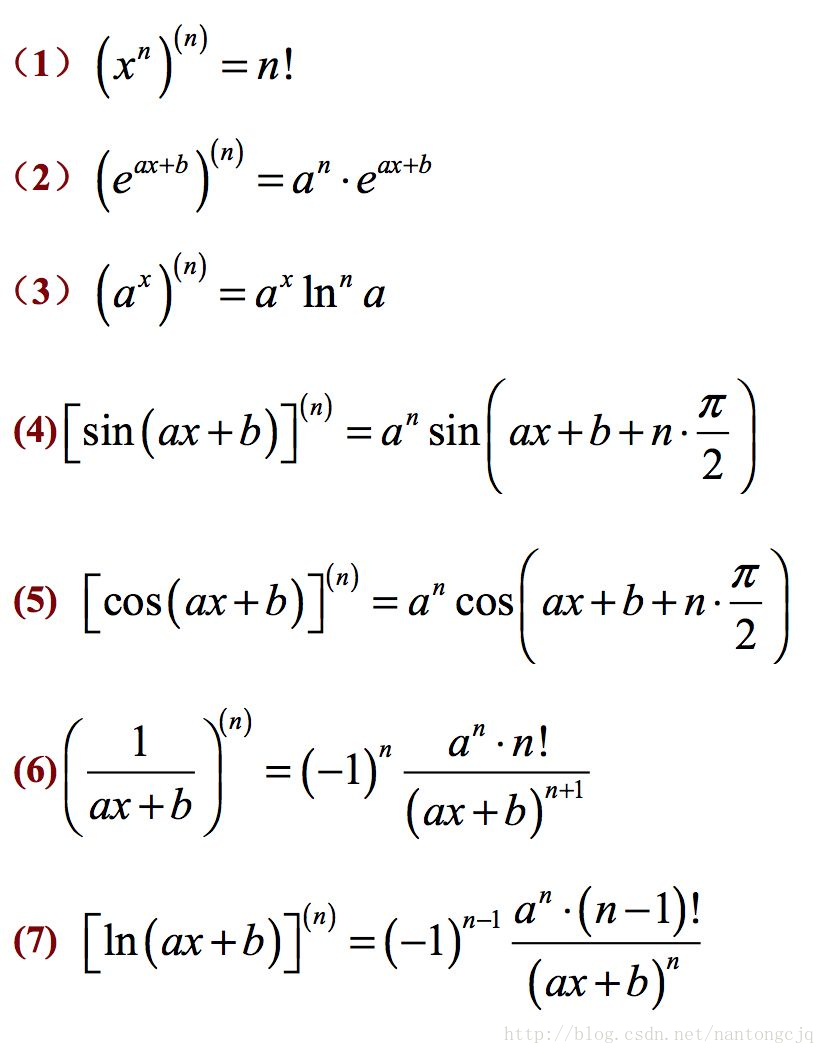
\includegraphics[width=0.50\linewidth]{../scoure/7.png}
      \end{center}
    \end{figure}
    \begin{figure}[!htb]
      \begin{center}
        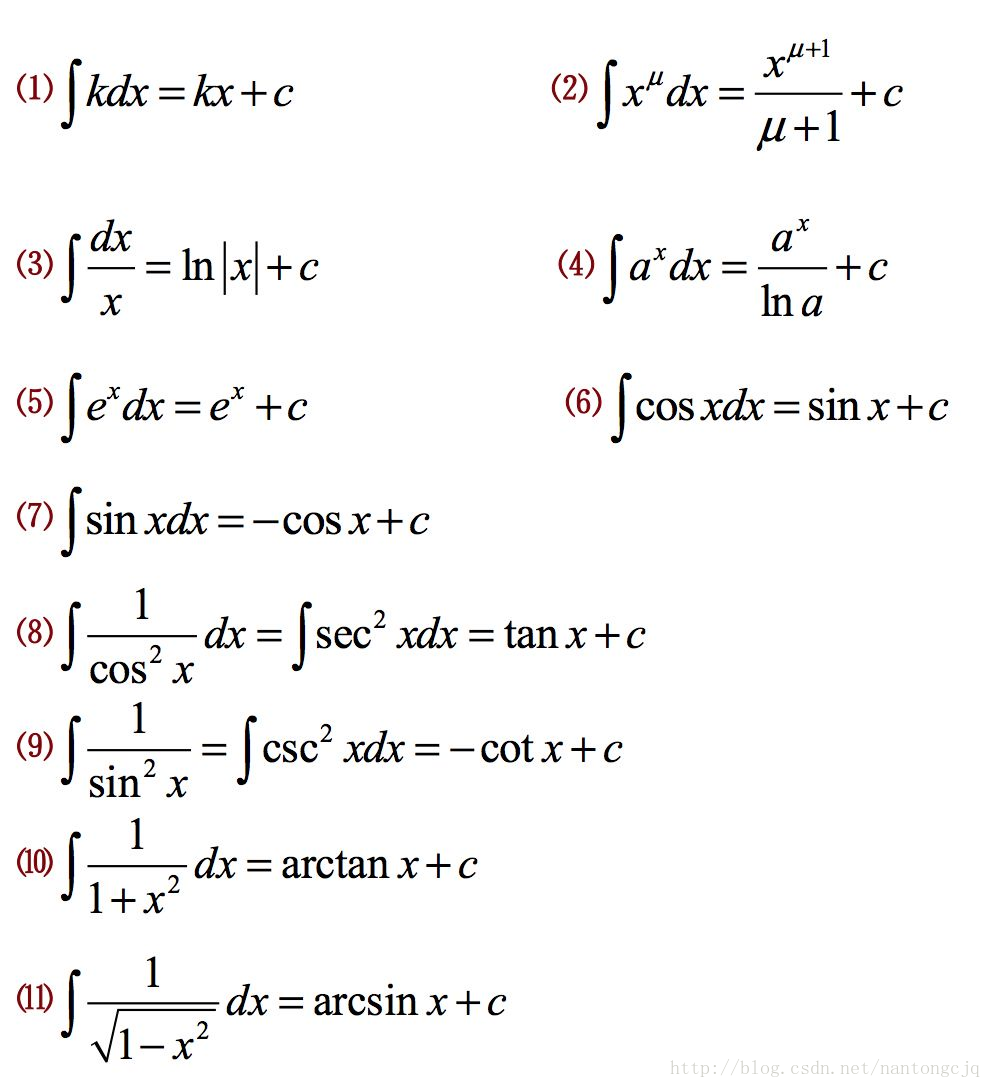
\includegraphics[width=0.50\linewidth]{../scoure/10.png}
      \end{center}
    \end{figure}
    \begin{figure}[!htb]
      \begin{center}
        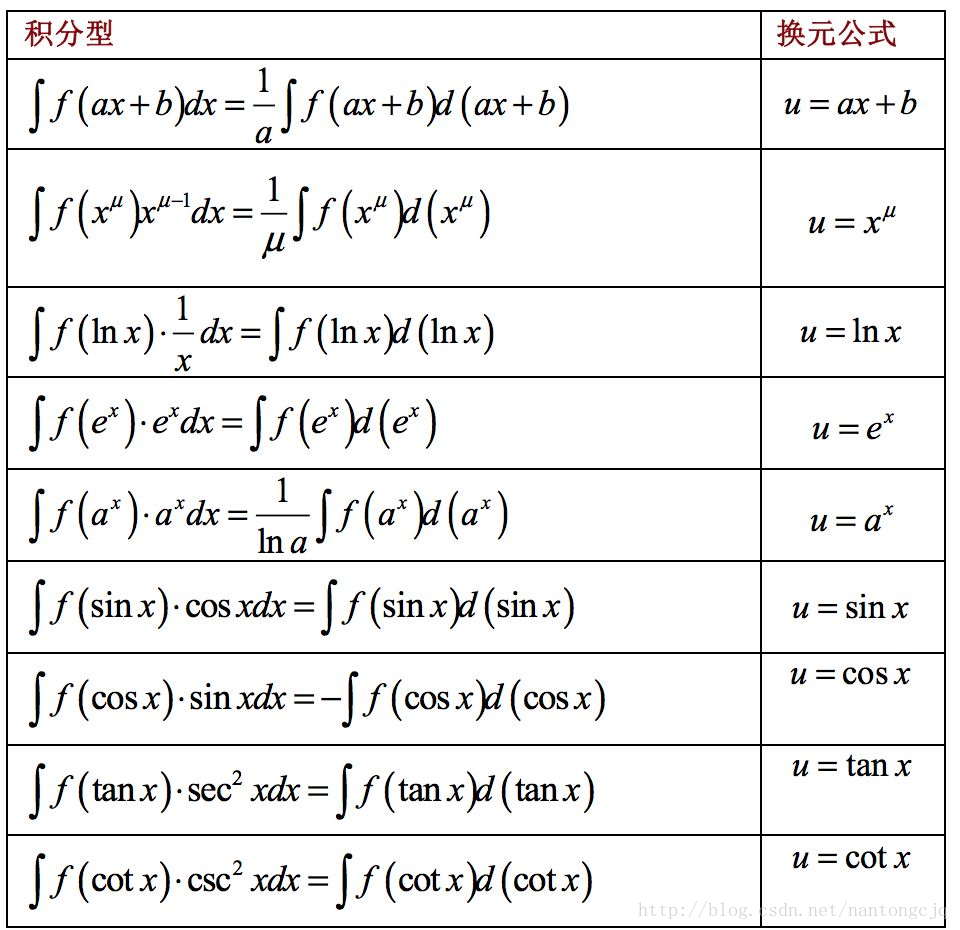
\includegraphics[width=0.50\linewidth]{../scoure/11.png}
      \end{center}
    \end{figure}
\newpage
啦啦啦
\end{CJK}
\end{document}
